\hsection{Installing PyCharm under Ubuntu Linux}%
%
\begin{figure}%
\centering%
%
\subfloat[][%
Installing \pycharm\ using the \bashil{snap install} command in a \pgls{terminal} opened with \ubuntuTerminal.%
\label{fig:installingPyCharmUbuntu01snapInstall}%
]{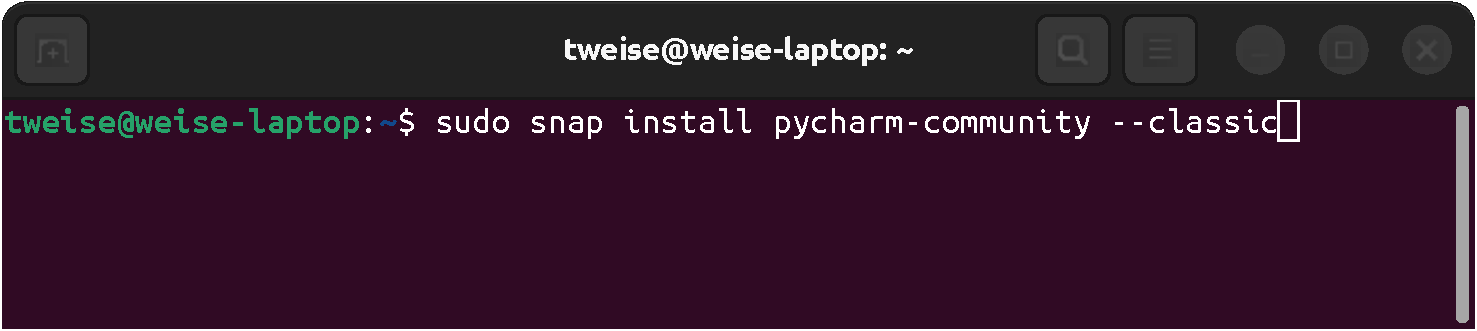
\includegraphics[width=0.7\linewidth]{\currentDir/installingPyCharmUbuntu01snapInstall}}%
%
\floatRowSep%
%
\subfloat[][%
This command requires the super user password, which we type in and then press~\keys{\enter}.%
\label{fig:installingPyCharmUbuntu02sudo}%
]{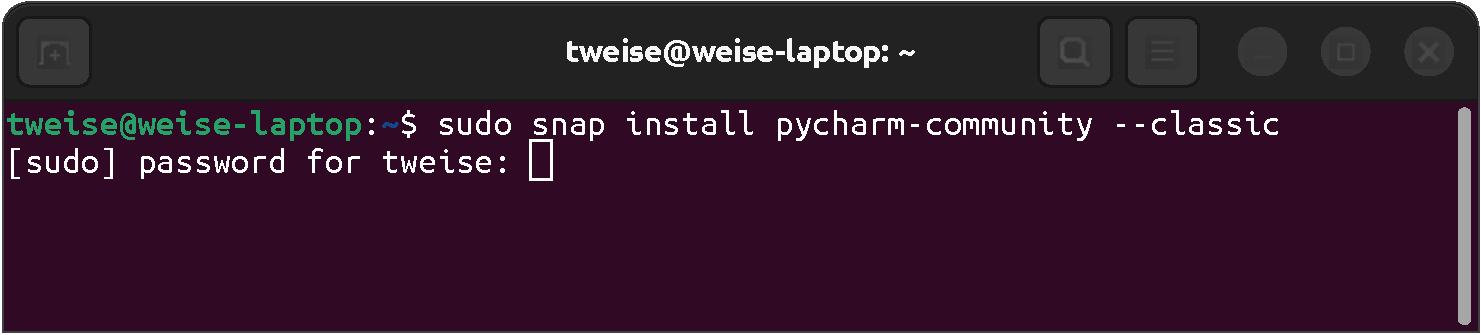
\includegraphics[width=0.7\linewidth]{\currentDir/installingPyCharmUbuntu02sudo}}%
%
\floatRowSep%
%
\subfloat[][%
The installation begins.%
\label{fig:installingPyCharmUbuntu03snapInstall}%
]{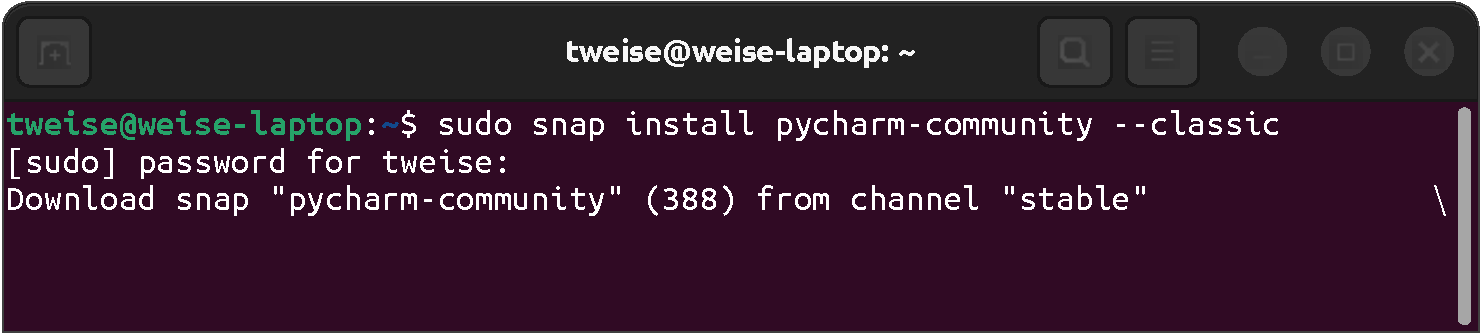
\includegraphics[width=0.7\linewidth]{\currentDir/installingPyCharmUbuntu03snapInstall}}%
%
\floatRowSep%
%
\subfloat[][%
The software package is downloaded.%
\label{fig:installingPyCharmUbuntu04snapInstall}%
]{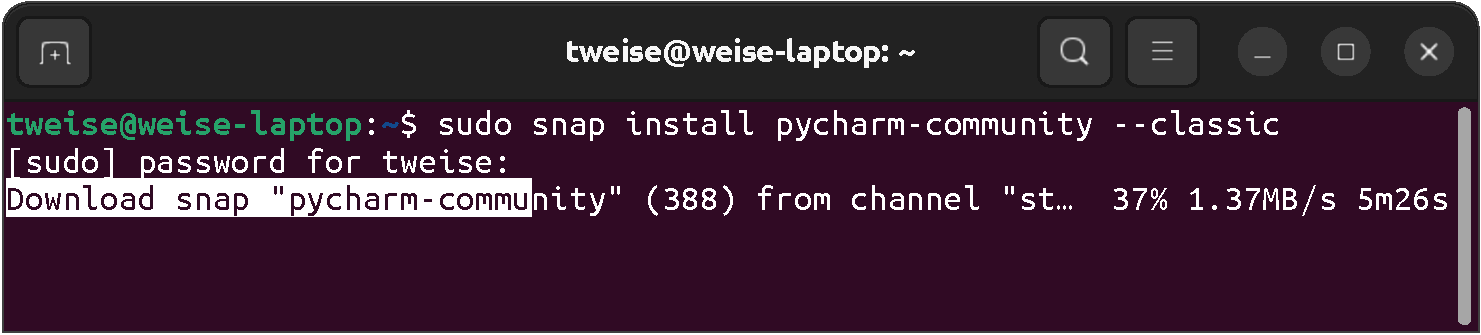
\includegraphics[width=0.7\linewidth]{\currentDir/installingPyCharmUbuntu04snapInstall}}%
%
\floatRowSep%
%
\subfloat[][%
The package is installed.%
\label{fig:installingPyCharmUbuntu05snapInstallFinished}%
]{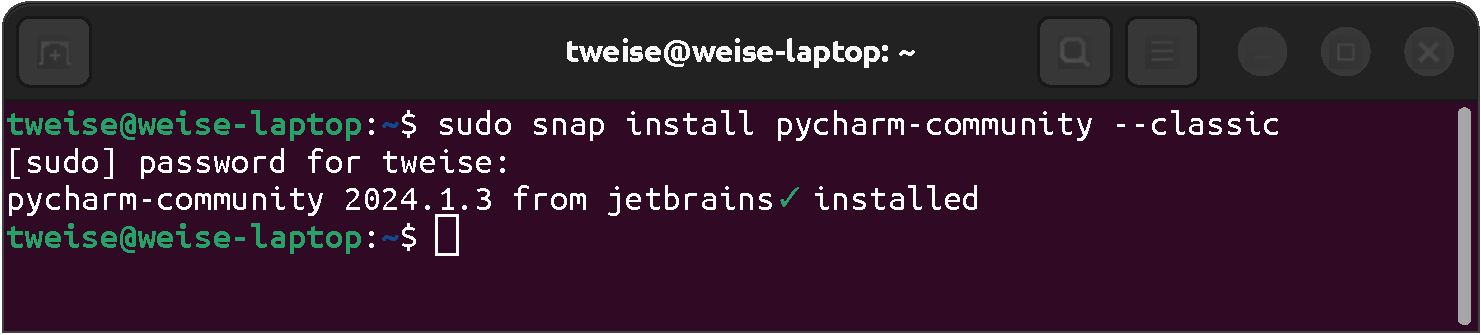
\includegraphics[width=0.7\linewidth]{\currentDir/installingPyCharmUbuntu05snapInstallFinished}}%
%
\floatRowSep%
%
\subfloat[][%
Open the launcher by pressing \OSwin\ and type in \bashil{pycharm} to find the \pycharm\ executable, then double-click it.%
\label{fig:installingPyCharmUbuntu06launcher}%
]{\tightbox{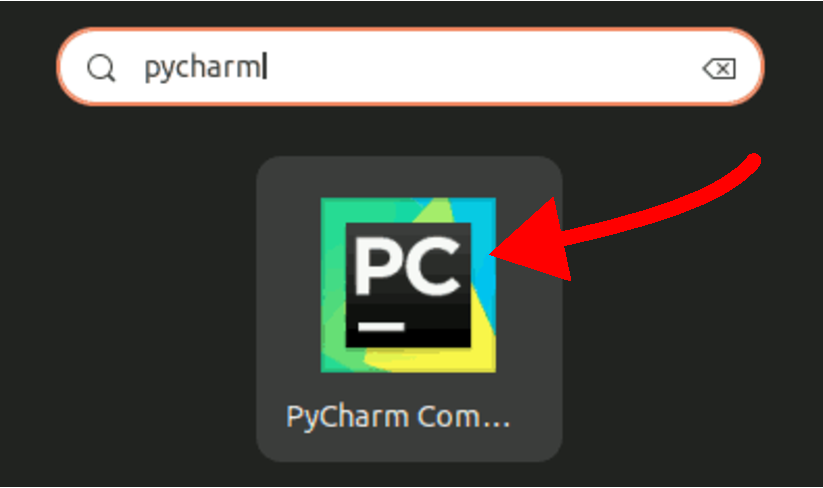
\includegraphics[height=3.1cm]{\currentDir/installingPyCharmUbuntu06launcher}}}%
%
\floatSep%
%
\subfloat[][%
The \pycharm\ welcome screen appears.%
\label{fig:installingPyCharmUbuntu07welcome}%
]{\tightbox{
\includegraphics[height=3.1cm]{\currentDir/installingPyCharmUbuntu07welcome}}}%
%
\floatSep%
%
\subfloat[][%
\pycharm\ has been started.%
\label{fig:installingPyCharmUbuntu08pycharm}%
]{\tightbox{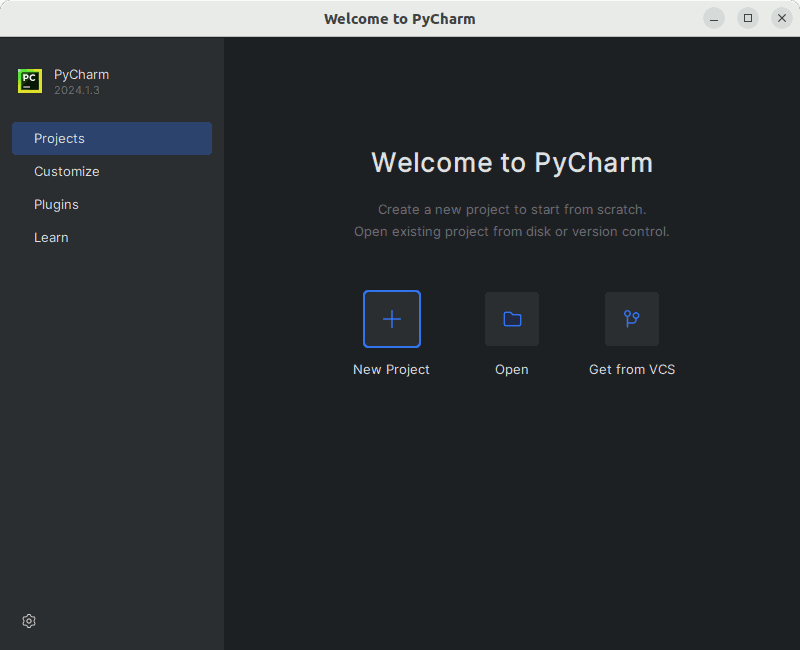
\includegraphics[height=3.1cm]{\currentDir/installingPyCharmUbuntu08pycharm}}}%
%
\caption{The installation steps of \pycharm\ under \ubuntu\ linux.}%
\label{fig:installingPyCharmUbuntu}%
\end{figure}%
%
\begin{sloppypar}%
\pycharm\ is available as Snap package under \ubuntu\ \linux~\cite{C2025SD,J2024PCPCE}.
The installation process is very easy and follows the steps illustrated in \cref{fig:installingPyCharmUbuntu}.
First, you open a \pgls{terminal} by pressing \ubuntuTerminal.
Then, enter the command \bashil{sudo snap install pycharm-community --classic} and hit~\keys{\enter}~(\cref{fig:installingPyCharmUbuntu01snapInstall}).
This installs the \pycharm\ software package and the necessary super user privileges are obtained via the pre-pended \pgls{sudo}, which will ask us to enter the root password, as sketched in \cref{fig:installingPyCharmUbuntu02sudo}.
Then, the installation process basically runs automatically.
Once it has completed (see \cref{fig:installingPyCharmUbuntu05snapInstallFinished}), you can press the \keys{\OSwin} key and type \bashil{pycharm} in the launcher window to find \pycharm~(\cref{fig:installingPyCharmUbuntu06launcher}).
A double-click will open \pycharm.%
\end{sloppypar}%
%
In the installation instructions for \microsoftWindows, now a user agreement~(\cref{fig:installingPyCharmWindows16running}) and data upload statement~(\cref{fig:installingPyCharmWindows17running}) need to be performed.
Since I already had \pycharm\ installed previously and probably already agreed/disagreed to them, respectively, these windows did not open in my current installation and I could not take screenshots of them.
If they open, then you can probably treat them exactly as suggested in the \microsoftWindows\ installation instructions \cref{sec:installingPyCharmWindows}.
Either way, we finally get \pycharm\ up and running and can begin our coding~(\cref{fig:installingPyCharmUbuntu08pycharm}).
%
\FloatBarrier%
\endhsection%
%
